% Created 2021-12-06 lun. 14:15
% Intended LaTeX compiler: pdflatex
\documentclass[10pt]{beamer}
\usepackage[utf8]{inputenc}
\usepackage[T1]{fontenc}
\usepackage{graphicx}
\usepackage{grffile}
\usepackage{longtable}
\usepackage{wrapfig}
\usepackage{rotating}
\usepackage[normalem]{ulem}
\usepackage{amsmath}
\usepackage{textcomp}
\usepackage{amssymb}
\usepackage{capt-of}
\usepackage{hyperref}
\usepackage{minted}
\setlength{\parskip}{5pt}
\newcommand{\footnoteframe}[1]{\footnote[frame]{#1}}
\addtobeamertemplate{footnote}{}{\vspace{2ex}}
\usepackage{tabularx}
\usetheme{Berkeley}
\author{Jay Morgan}
\date{}
\title{Programming Level-up}
\subtitle{An Introduction to Pandas}
\hypersetup{
 pdfauthor={Jay Morgan},
 pdftitle={Programming Level-up},
 pdfkeywords={},
 pdfsubject={},
 pdfcreator={Emacs 27.1 (Org mode 9.4.6)}, 
 pdflang={English}}
\begin{document}

\maketitle
\begin{frame}{Outline}
\tableofcontents
\end{frame}


\section{Pandas}
\label{sec:org89153d3}

\subsection{Introduction}
\label{sec:orgd4fef91}

\begin{frame}[label={sec:org4513bde}]{What is Pandas?}
\begin{center}
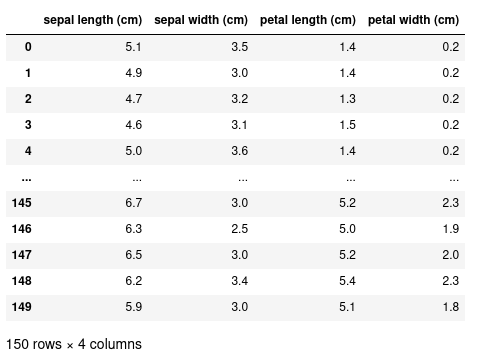
\includegraphics[width=0.5\textwidth]{./images/pandas.jpg}
\end{center}

\begin{itemize}
\item Pandas a library to make the representation and manipulation of tabular data
easier in Python.
\item A table of data is called a 'Dataframe' that consists of named columns and
(optionally) named rows.
\item \url{https://pandas.pydata.org/}
\end{itemize}
\end{frame}

\begin{frame}[label={sec:org8264db7},fragile]{Installing and importing pandas}
 To install pandas, we can either use conda:

\begin{minted}[frame=lines,linenos=true,firstnumber=last,fontsize=\footnotesize,xleftmargin=15pt,numbersep=8pt]{bash}
conda install pandas
\end{minted}

or with pip:

\begin{minted}[frame=lines,linenos=true,firstnumber=last,fontsize=\footnotesize,xleftmargin=15pt,numbersep=8pt]{bash}
pip install pandas
\end{minted}

After pandas has been installed. We shall import it into our scripts (using the
common convention of aliasing the library as pd):

\begin{minted}[frame=lines,linenos=true,firstnumber=last,fontsize=\footnotesize,xleftmargin=15pt,numbersep=8pt]{python}
import pandas as pd
\end{minted}
\end{frame}

\begin{frame}[label={sec:org24d7eb7},fragile]{Creating a dataframe}
 Now that pandas has been successfully imported, we're ready to create and
manipulate our own dataframes. To create a dataframe, we first need to organise
our data in appropriate format. Perhaps one of the most simple formats for this
data is a dictionary, where each value is a list:

\begin{minted}[frame=lines,linenos=true,firstnumber=last,fontsize=\footnotesize,xleftmargin=15pt,numbersep=8pt]{python}
data = {"col1": [1, 2], "col2": [3, 4]}
\end{minted}

We see that each 'key' is the representation of a column of data, and the value
of this key is a list of data for this column. To convert this data to a
dataframe, we need only to call the DataFrame class:

\begin{minted}[frame=lines,linenos=true,firstnumber=last,fontsize=\footnotesize,xleftmargin=15pt,numbersep=8pt]{python}
df = pd.DataFrame(data)
\end{minted}
\end{frame}

\begin{frame}[label={sec:org9900b09},fragile]{Creating a dataframe}
 \texttt{df} (dataframe for short) is now our representation of the dataframe:

\begin{center}
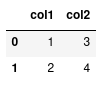
\includegraphics[width=0.2\textwidth]{images/simple_dataframe.png}
\end{center}

We see that each column is named using the keys in our \texttt{data} dictionary, and the
values of the column correspond to the elements in the list. To the left of the
dataframe we have a numerical index starting at 0.
\end{frame}

\begin{frame}[label={sec:org4ee206e},fragile]{Access elements in our dataframe}
 Extracting particular values from this dataframe can be accomplished using the
\texttt{loc} and \texttt{iloc} class methods. First let's look at using \texttt{loc}, and later on we'll
investigate the differences between these two methods.

Let's say we want to get all the data for the first row of our dataframe:

\begin{minted}[frame=lines,linenos=true,firstnumber=last,fontsize=\footnotesize,xleftmargin=15pt,numbersep=8pt]{python}
df.loc[0]
\end{minted}

\begin{center}
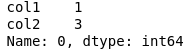
\includegraphics[scale=0.5]{images/series.png}
\end{center}

This returns a 'Series', which is just a representation of a vector of data.
\end{frame}

\begin{frame}[label={sec:orgd3a1bc5},fragile]{Access elements in our dataframe}
 To access a single value from this series, we can specify the column name:

\begin{minted}[frame=lines,linenos=true,firstnumber=last,fontsize=\footnotesize,xleftmargin=15pt,numbersep=8pt]{python}
df.loc[0]["col1"]  # returns one
\end{minted}

Or, we can more simply add the column name into the \texttt{loc}:

\begin{minted}[frame=lines,linenos=true,firstnumber=last,fontsize=\footnotesize,xleftmargin=15pt,numbersep=8pt]{python}
df.loc[0, "col1"]
\end{minted}

If we wanted to retrieve a subset of columns, we supply a list of column names:

\begin{minted}[frame=lines,linenos=true,firstnumber=last,fontsize=\footnotesize,xleftmargin=15pt,numbersep=8pt]{python}
df.loc[0, ["col1", "col2"]]
\end{minted}
\end{frame}

\begin{frame}[label={sec:orgb998a5b},fragile]{Access elements in our dataframe}
 We can also use the slice notation to access multiple rows:

\begin{minted}[frame=lines,linenos=true,firstnumber=last,fontsize=\footnotesize,xleftmargin=15pt,numbersep=8pt]{python}
df.loc[0:2, "col1"]
\end{minted}

This retrieves the values in \texttt{col1}.

Or if we just wanted to get the entire column of data, we could instead do:

\begin{minted}[frame=lines,linenos=true,firstnumber=last,fontsize=\footnotesize,xleftmargin=15pt,numbersep=8pt]{python}
df["col1"]
\end{minted}
\end{frame}

\subsection{Manipulating data}
\label{sec:org2627b4e}

\begin{frame}[label={sec:org37f3120},fragile]{Reading a CSV file}
 Instead of manually constructing our data and then passing it to a DataFrame, we
can use pandas to read directly from a CSV file and return a DataFrame:

Let's say we have a CSV file of measurements of Iris flowers called \texttt{iris.csv}. We
can read this CSV file using the \texttt{pd.read\_csv} method.

\begin{minted}[frame=lines,linenos=true,firstnumber=last,fontsize=\footnotesize,xleftmargin=15pt,numbersep=8pt]{python}
df = pd.read_csv("iris.csv")
\end{minted}

\begin{center}
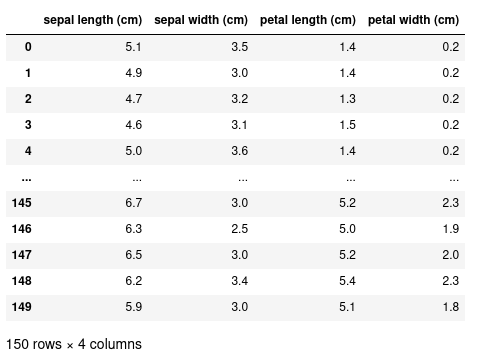
\includegraphics[width=0.5\textwidth]{images/pandas.jpg}
\end{center}
\end{frame}

\begin{frame}[label={sec:orgb1c6d6a},fragile]{Selecting a subset of data}
 With this more complex dataset, we can use more fancy methods of indexing. For
example, let's select all the rows where the sepal length is less than 5 cm.

\begin{minted}[frame=lines,linenos=true,firstnumber=last,fontsize=\footnotesize,xleftmargin=15pt,numbersep=8pt]{python}
df[df["sepal length (cm)"] < 5]
\end{minted}

\begin{center}
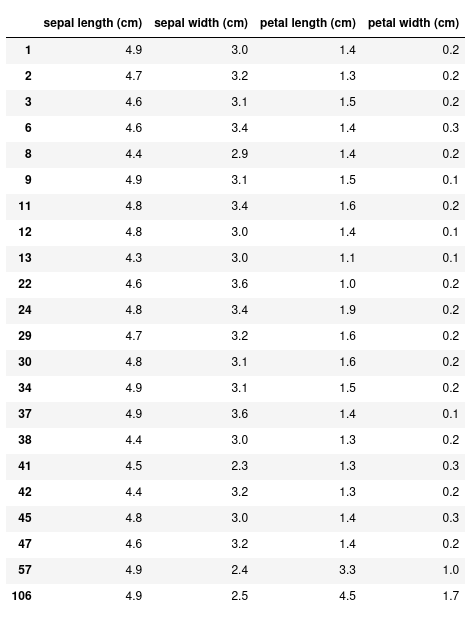
\includegraphics[width=0.4\textwidth]{images/subset.png}
\end{center}

Instead of the 150 rows we had before, this returns just 22. We can also specify
only the columns we want with this conditional expression:

\begin{minted}[frame=lines,linenos=true,firstnumber=last,fontsize=\footnotesize,xleftmargin=15pt,numbersep=8pt]{python}
df[df["sepal length (cm)"] < 5]["sepal width (cm)"]
\end{minted}
\end{frame}

\begin{frame}[label={sec:orgee6cf72},fragile]{Creating new columns}
 We can add new columns to this dataset by using the assignment operator. In this
example, we're creating a new column called 'sepal sum' to be the sum of both
the 'sepal width' and 'sepal length':

\begin{minted}[frame=lines,linenos=true,firstnumber=last,fontsize=\footnotesize,xleftmargin=15pt,numbersep=8pt]{python}
df["sepal sum"] = df["sepal width (cm)"] + df["sepal length (cm)"]
\end{minted}

\begin{center}
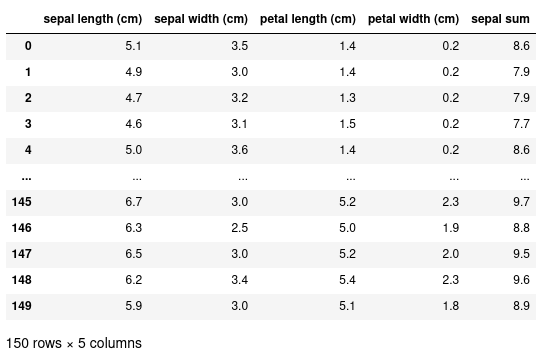
\includegraphics[width=0.5\textwidth]{images/new-column.png}
\end{center}
\end{frame}

\subsection{Inspecting our data}
\label{sec:org5cfa47f}

\begin{frame}[label={sec:org6a6989a},fragile]{Shape of the data}
 We can also further see that our new column has been added by inspecting the
\texttt{shape} of the data.

\begin{minted}[frame=lines,linenos=true,firstnumber=last,fontsize=\footnotesize,xleftmargin=15pt,numbersep=8pt]{python}
df.shape
\end{minted}

\begin{verbatim}
(150, 5)
\end{verbatim}

This returns a tuple corresponding to the number of rows (150) and the number of
columns (5).
\end{frame}

\begin{frame}[label={sec:org5eeff61},fragile]{Getting the names of columns}
 To find out what the names of the columns are we can use the \texttt{columns} attribute:

\begin{minted}[frame=lines,linenos=true,firstnumber=last,fontsize=\footnotesize,xleftmargin=15pt,numbersep=8pt]{python}
df.columns
\end{minted}

\begin{verbatim}
Index(['sepal length (cm)', 'sepal width (cm)', 'petal length (cm)',
       'petal width (cm)', 'sepal sum'],
      dtype='object')
\end{verbatim}

This returns an Index that can itself be indexed in the usual way:

\begin{minted}[frame=lines,linenos=true,firstnumber=last,fontsize=\footnotesize,xleftmargin=15pt,numbersep=8pt]{python}
df.columns[0]
\end{minted}

\begin{verbatim}
'sepal length (cm)'
\end{verbatim}
\end{frame}

\begin{frame}[label={sec:org1086120},fragile]{Head/tail}
 We can get the first/last few rows of the data using the \texttt{.head()} or \texttt{.tail()}
methods. These take an optional argument specifying the number of rows to
view. By default, it will show 10 rows.

\begin{minted}[frame=lines,linenos=true,firstnumber=last,fontsize=\footnotesize,xleftmargin=15pt,numbersep=8pt]{python}
df.head()  # shows the first 10 rows
df.head(5) # shows the first 5 rows

df.tail()  # shows the last 10 rows
df.tail(5) # shows the last 5 rows
\end{minted}
\end{frame}


\subsection{Operations}
\label{sec:org13709ea}

\begin{frame}[label={sec:org6ff4558},fragile]{Operations on data}
 Pandas comes with a few standard methods to perform some basic operations. For
example, you can calculate the mean of a column:

\begin{minted}[frame=lines,linenos=true,firstnumber=last,fontsize=\footnotesize,xleftmargin=15pt,numbersep=8pt]{python}
df["sepal length (cm)"].mean()
\end{minted}

And you can use the \texttt{apply()} method to apply a function to every element
(i.e. map a function to every element):

\begin{minted}[frame=lines,linenos=true,firstnumber=last,fontsize=\footnotesize,xleftmargin=15pt,numbersep=8pt]{python}
df["sepal length (cm)"].apply(lambda x: x * 2)
\end{minted}

Apply takes a function as an argument, and here we're using an anonymous
(unnamed function) using a lambda expression
\url{https://docs.python.org/3/tutorial/controlflow.html\#lambda-expressions}

This lambda expression will double its input, and therefore applying this
function to every element will double all values in 'sepal length (cm)'.
\end{frame}

\begin{frame}[label={sec:orgb9ab985},fragile]{Merge}
 Many pandas dataframes can be combined together using the \texttt{concat} method that
requires a list of dataframes as input.

\begin{minted}[frame=lines,linenos=true,firstnumber=last,fontsize=\footnotesize,xleftmargin=15pt,numbersep=8pt]{python}
data1 = pd.DataFrame({"col1": [0, 1], "col2": [0, 1]})
data2 = pd.DataFrame({"col1": [2, 3], "col2": [2, 3]})

combined = pd.concat([data1, data2])
\end{minted}

\begin{center}
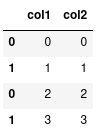
\includegraphics[width=0.2\textwidth]{images/combined.png}
\end{center}
\end{frame}

\begin{frame}[label={sec:org4748934},fragile]{More on indexing}
 \begin{center}
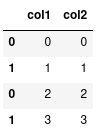
\includegraphics[width=0.2\textwidth]{images/combined.png}
\end{center}

Notice how the indexes are repeated. We can also verify this using the \texttt{.index}
attribute:

\begin{minted}[frame=lines,linenos=true,firstnumber=last,fontsize=\footnotesize,xleftmargin=15pt,numbersep=8pt]{python}
combined.index
\end{minted}

\begin{verbatim}
Int64Index([0, 1, 0, 1], dtype='int64')
\end{verbatim}

We can see two '0's and two '1's. Normally, this is not a problem, but it does
have an effect on when we index our data with \texttt{loc}.
\end{frame}

\begin{frame}[label={sec:org1887ef4},fragile]{More on indexing}
 \begin{minted}[frame=lines,linenos=true,firstnumber=last,fontsize=\footnotesize,xleftmargin=15pt,numbersep=8pt]{python}
combined.loc[1]
\end{minted}

\begin{center}
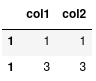
\includegraphics[width=0.2\textwidth]{images/indexing.png}
\end{center}

Notice how \texttt{loc} has returned two rows because it sees two rows with the index
label of 1. If instead we simply meant: give me the second row we should use
\texttt{iloc}:

\begin{minted}[frame=lines,linenos=true,firstnumber=last,fontsize=\footnotesize,xleftmargin=15pt,numbersep=8pt]{python}
combined.iloc[1]
\end{minted}

Which will give us the desired outcome.
\end{frame}

\begin{frame}[label={sec:org82b2dcd},fragile]{Resetting indexes}
 Alternatively we can reset the index labels:

\begin{minted}[frame=lines,linenos=true,firstnumber=last,fontsize=\footnotesize,xleftmargin=15pt,numbersep=8pt]{python}
combined.reset_index()
\end{minted}

\begin{center}
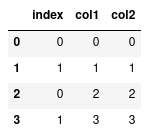
\includegraphics[width=0.2\textwidth]{images/reset-index.png}
\end{center}

This will compute a new series of indexes for our data, and then using \texttt{loc} again
will only return the one row.
\end{frame}

\begin{frame}[label={sec:org2f66229},fragile]{Resetting indexes}
 To save the result of \texttt{reset\_index()} we need to overwrite our original data:

\begin{minted}[frame=lines,linenos=true,firstnumber=last,fontsize=\footnotesize,xleftmargin=15pt,numbersep=8pt]{python}
combined = combined.reset_index()
\end{minted}

Or specify \texttt{inplace}:

\begin{minted}[frame=lines,linenos=true,firstnumber=last,fontsize=\footnotesize,xleftmargin=15pt,numbersep=8pt]{python}
combined.reset_index(inplace=True)
\end{minted}
\end{frame}

\subsection{Different types of data}
\label{sec:org844512b}

\begin{frame}[label={sec:org0184a77},fragile]{Categorical data}
 So far, we've only seen numerical data. One of the advantages of using pandas
for tabular data is that we can represent various other types of data that makes
our manipulation and operations on different data types simpler. For example, we
can represent 'categorical data' where there is a finite set of values or
categories.

\begin{minted}[frame=lines,linenos=true,firstnumber=last,fontsize=\footnotesize,xleftmargin=15pt,numbersep=8pt]{python}
df = pd.DataFrame({"col1": ["a", "b", "c", "a"],
		   "col2": [1, 2, 5, 4]})
\end{minted}

Right now, \texttt{df} is simply representing 'col1' as strings, but we can change the
representation to categorical elements with:

\begin{minted}[frame=lines,linenos=true,firstnumber=last,fontsize=\footnotesize,xleftmargin=15pt,numbersep=8pt]{python}
df["col1"] = df["col1"].astype("category")
\end{minted}
\end{frame}


\begin{frame}[label={sec:org7496350},fragile]{Categorical data}
 With categorical data, we can perform operations on these groups a lot quicker
than if we were just to represent them on strings. For instance, lets compute
the sum of 'col2' for each group.

\begin{minted}[frame=lines,linenos=true,firstnumber=last,fontsize=\footnotesize,xleftmargin=15pt,numbersep=8pt]{python}
df.groupby("col1").sum()
\end{minted}

\begin{center}
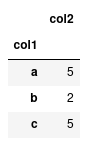
\includegraphics[width=0.1\textwidth]{images/categorical.png}
\end{center}

If we have lots of data, having 'col1' \texttt{astype('category')} will be a lot more
computationally efficient than leaving them as strings.
\end{frame}

\begin{frame}[label={sec:orgcf50151},fragile]{Dates and times}
 If you have a column that represents a date or time, you can convert that column
to a true datetime representation with \texttt{pd.to\_datetime}

\begin{minted}[frame=lines,linenos=true,firstnumber=last,fontsize=\footnotesize,xleftmargin=15pt,numbersep=8pt]{python}
df = pd.DataFrame({"col1": ["2002/01/30", "2010/05/16"]})
df["col1"] = pd.to_datetime(df["col1"])
\end{minted}

In addition to make indexing by dates a lot faster, it also provides us with
some convienant methods to extract particular components from the data. Such as
the year:

\begin{minted}[frame=lines,linenos=true,firstnumber=last,fontsize=\footnotesize,xleftmargin=15pt,numbersep=8pt]{python}
df["col1"].dt.year # or df["col1"].dt.month etc
\end{minted}

\begin{center}
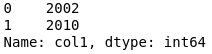
\includegraphics[width=0.3\textwidth]{images/year.png}
\end{center}
\end{frame}
\end{document}
